\documentclass[aspectratio=169,10pt]{beamer}
\usetheme{default}
\usecolortheme{default}
\setbeamertemplate{navigation symbols}{}
\setbeamertemplate{footline}{\hfill\scriptsize Daniel Murnane \quad quirkml status, 17 October 2026\hspace{1em}\insertframenumber\hspace{0.5em}\vspace{0.4em}}
\setbeamerfont{frametitle}{size=\large}
\setbeamercolor{frametitle}{fg=black}
\usepackage{booktabs}
\usepackage{tikz}
\usetikzlibrary{positioning,arrows.meta}
\usepackage{graphicx}
\newcommand{\figdir}{/global/cfs/cdirs/m4958/usr/danieltm/ColliderML/quirkml/docs/talks/2026-10-17/figs}
\newcommand{\fig}[2]{\IfFileExists{\figdir/#1.pdf}{\includegraphics[#2]{\figdir/#1.pdf}}{\fbox{\parbox{0.4\linewidth}{\centering\small figure \detokenize{#1} missing}}}}
\renewcommand{\arraystretch}{1.15}

\begin{document}

\begin{frame}
\vspace{2em}
{\Large Quirks in ColliderML: simulation at scale and first ML tracking}\\[1em]
Daniel Murnane\\[0.3em]
{\small quirkml status, 17 October 2026}\\[2em]
\small
\begin{itemize}
\item Quirk-gen events through the ColliderML chain, in runs, multi-threaded, packaged as published ColliderML datasets
\item Pilots at $\mu = 0$ and $\mu = 10$; simulation cost across the $(m, \Lambda)$ grid
\item An ACTS-based evaluator for quirk tracks; first GNN and MaskFormer results at $m = 200$ GeV, $\Lambda = 774$ eV
\end{itemize}
\end{frame}

\begin{frame}{The chain}
\centering
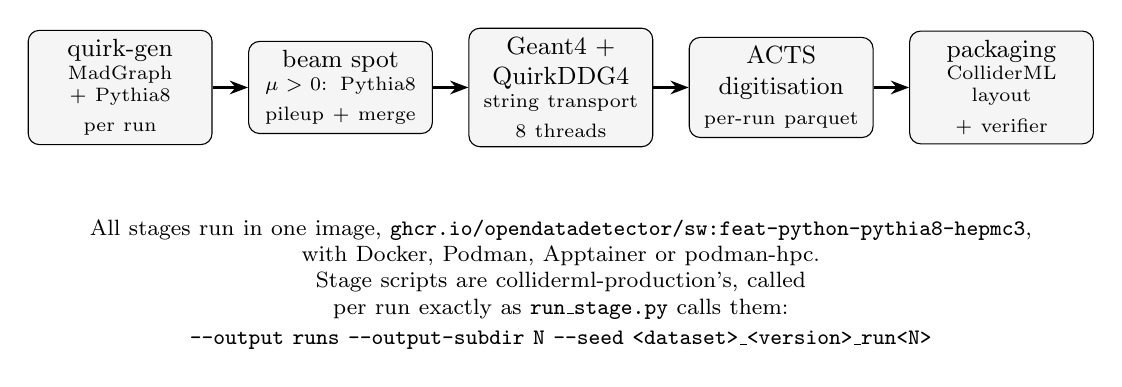
\begin{tikzpicture}[node distance=0.35cm and 0.45cm, every node/.style={font=\small},
  box/.style={draw, rounded corners, align=center, minimum height=1.1cm, text width=2.1cm, fill=gray!8}, >=Stealth]
\node[box] (gen) {quirk-gen\\\scriptsize MadGraph + Pythia8\\per run};
\node[box, right=of gen] (s1) {beam spot\\\scriptsize $\mu>0$: Pythia8\\pileup + merge};
\node[box, right=of s1] (sim) {Geant4 + QuirkDDG4\\\scriptsize string transport\\8 threads};
\node[box, right=of sim] (digi) {ACTS digitisation\\\scriptsize per-run parquet};
\node[box, right=of digi] (pack) {packaging\\\scriptsize ColliderML layout\\+ verifier};
\foreach \a/\b in {gen/s1, s1/sim, sim/digi, digi/pack} \draw[->, thick] (\a) -- (\b);
\node[below=0.8cm of sim, align=center, text width=12cm] (img) {\footnotesize All stages run in one image, \texttt{ghcr.io/opendatadetector/sw:feat-python-pythia8-hepmc3}, with Docker, Podman, Apptainer or podman-hpc.\\
Stage scripts are colliderml-production's, called per run exactly as \texttt{run\_stage.py} calls them:\\
\texttt{--output runs --output-subdir N --seed <dataset>\_<version>\_run<N>}};
\end{tikzpicture}

\vspace{0.5em}
\footnotesize
\resizebox{\linewidth}{!}{%
\begin{tabular}{lll}
\toprule
 & colliderml-production & quirkml \\
\midrule
layout & \texttt{<campaign>/<dataset>/<version>/runs/<N>} & same, campaign \texttt{quirks}, on CFS \texttt{simulation/} \\
seeds & hashed \texttt{<dataset>\_<version>\_run<N>}, every stage & same; quirk-gen gets the same integer \\
MadGraph & process built once, copied per run & quirk-gen's process built once, copied per run \\
parallelism & \texttt{threads} per run, \texttt{runs\_per\_node} & \texttt{sim\_threads}, \texttt{--parallel K}, Slurm/HTCondor examples \\
packaging & \texttt{package\_native\_parquet.py} + verifier & same scripts, unchanged \\
\bottomrule
\end{tabular}}
\end{frame}

\begin{frame}{QuirkDDG4 is now multi-threaded}
\centering
\fig{mt_validation}{width=0.68\linewidth}

\vspace{0.1em}
\scriptsize
\begin{columns}[T]
\column{0.48\textwidth}
The ported Athena plugin kept each pair's string on the quirk particle definition, which Geant4 shares between worker threads, so it ran on one thread. Now the string state is per thread, the stacking action is installed on every worker, and strings are cleared at the start of each event.
\column{0.48\textwidth}
$m = 200$ GeV, $\Lambda = 774$ eV, $\mu = 0$:
\begin{itemize}
\item 1 thread: 20/20 events identical to the old plugin
\item 1 vs 8 threads, same 400 events: quirk hits/event 32.49 vs 32.42 (paired $-0.07 \pm 0.16$); 2095 s vs 369 s
\item plain ddsim without quirks is not reproducible event by event across thread counts either (11/40)
\end{itemize}
\end{columns}
\end{frame}

\begin{frame}{Pilots: 8 runs $\times$ 500 events at $\mu = 0$ and $\mu = 10$}
\begin{columns}[T]
\column{0.55\textwidth}
\centering
\fig{pilot_stage_times}{width=\linewidth}

\scriptsize
$m = 400$ GeV, $\Lambda = 1$ keV. Wall time per stage, 8 runs at once on one node. Simulation ran as one debug-queue job, one Slurm task per run (\texttt{colliderml/batch/slurm\_runs.sh}).
\column{0.43\textwidth}
\footnotesize
\resizebox{\linewidth}{!}{%
\begin{tabular}{lcc}
\toprule
 & $\mu = 0$ & $\mu = 10$ \\
\midrule
events & 4000 & 4000 \\
unique ids and momenta & yes & yes \\
verifier & PASS & PASS \\
quirk hits / event$^*$ & $30.05 \pm 0.24$ & $30.19 \pm 0.26$ \\
tracker hits / event & 3874 & 14082 \\
sim. core-s / event & 7 & 14 \\
peak memory, 8 runs & n/a & 65 GB \\
disk / event & 1.7 MB & 6.3 MB \\
\bottomrule
\end{tabular}}

\vspace{0.3em}
\scriptsize $^*$ a hit counts if any of its truth particles is a quirk. Tracker hits: median.
\end{columns}
\end{frame}

\begin{frame}{Hits per event}
\centering
\fig{quirk_hits_per_event}{width=0.82\linewidth}

\vspace{0.2em}
\begin{columns}[T]
\column{0.42\textwidth}
\centering
\fig{hits_per_event}{width=0.95\linewidth}
\column{0.52\textwidth}
\footnotesize
\vspace{1.5em}
$m = 400$ GeV, $\Lambda = 1$ keV. Quirk hits do not change with pileup: $+0.13 \pm 0.35$ per event from $\mu = 0$ to $\mu = 10$. Per-run means are consistent within their errors.
\end{columns}
\end{frame}

\begin{frame}{Three regimes of the string}
\centering
\fig{evd_regimes}{height=0.78\textheight}

\footnotesize
$m = 175$ GeV. Separated trajectories ($\Lambda \le 278$ eV), interleaved ($464$-$1292$ eV), unresolved pair ($\ge 2154$ eV).
\end{frame}

\begin{frame}{Simulation cost across the grid}
\begin{columns}[c]
\column{0.44\textwidth}
\centering
\fig{cost_vs_lambda}{width=\linewidth}
\column{0.54\textwidth}
\centering
\fig{quirk_hits_vs_lambda}{width=\linewidth}
\end{columns}
\scriptsize
\begin{columns}[T]
\column{0.48\textwidth}
\begin{itemize}
\item 15 points $\times$ 100 events, 8 threads per run, start-up removed.
\item 3 core-s/event at $\Lambda \le 278$ eV, 300 at 10 keV ($m = 175$ GeV), while hits per quirk barely change.
\item At 10 keV mass matters: 400 ($m = 50$) and 185 ($m = 300$) core-s/event.
\end{itemize}
\column{0.48\textwidth}
\begin{itemize}
\item Grid average at $\mu = 0$: about 51 core-s/event, so about 9000 events per node-hour. The 6 and 10 keV rows are about 80\% of it.
\item $\mu = 60$ at 774 eV: 52 core-s/event in simulation, 65 in all; 29 MB/event.
\end{itemize}
\end{columns}
\end{frame}

\begin{frame}{What about 1000 node-hours could produce}
\footnotesize
\centering
\begin{tabular}{llrrr}
\toprule
set & content & events & node-hours & disk \\
\midrule
A & $\mu = 0$, every grid point ($11 \times 10$), 20k each & 2.2 M & $\sim$245 & 4.2 TB \\
B & $\mu = 0$, $m = 200$ GeV, $\Lambda = 774$ eV, scaled to 1 M & 1.0 M & $\sim$20 & 1.9 TB \\
C & $\mu = 60$, every grid point, 2k each & 220 k & $\sim$55 & 6.4 TB \\
D & $\mu = 60$, 3 training points ($\Lambda = 278, 774, 2154$ eV), 100k each & 300 k & $\sim$50 & 8.7 TB \\
\midrule
 & total & 3.7 M & $\sim$370 & 21 TB \\
\bottomrule
\end{tabular}

\vspace{1em}
\raggedright
\begin{itemize}
\item Datasets go to \texttt{/global/cfs/cdirs/m4958/data/ColliderML/simulation/quirks/} (m4958 CFS: 303 of 512 TB used), as \texttt{<dataset>/<version>/\{runs,parquet\}}. The pilots, the 20k tracking set and the cost sets are moved there.
\item CPU on m4958 (regular queue), GPU on m5386.
\item Open: the mix of sets, and how much of the remaining $\sim$600 node-hours to spend now.
\end{itemize}
\end{frame}

\begin{frame}{Tracking evaluation: ACTS, proto-track level}
\begin{columns}[T]
\column{0.45\textwidth}
\footnotesize
The ML-Tracking-Review evaluator (pyacts 48), copied into \texttt{quirkml/tracking/}. Metrics:
\begin{enumerate}
\item quirk track efficiency, per quirk (figure of merit): charged, primary, $\ge 3$ hits, no $p_T$/$\eta$ cut
\item quirk event efficiency: both quirks matched
\item technical efficiency ($p_T > 1$ GeV, $|\eta| < 3$, prompt, $\ge 7$ hits), with and without quirks
\item fake and duplicate rates
\end{enumerate}
Matching: very loose (50\% of hits, double matching) and tight (90\%). The Kalman-fit level assumes helices: 0.6\% quirk efficiency even for truth predictions, so it is not used.
\column{0.53\textwidth}
\footnotesize
Validation on $m = 400$ GeV (4000 events; very loose / tight):

\vspace{0.3em}
\resizebox{\linewidth}{!}{%
\begin{tabular}{lcccc}
\toprule
prediction & quirk & q. event & tech. & fake \\
\midrule
truth & 1 / 1 & 1 / 1 & 1 / 1 & 0 \\
quirks split by time & 1 / 0 & 1 / 0 & 1 / 0.90 & 0.002 \\
60\% quirk hits dropped & 0 & 0 & 0.90 & 0.003 \\
quirks kept with p = 0.5 & 0.50 & 0.24 & 0.95 & 0 \\
nothing assigned & 0 & 0 & 0 & n/a \\
\bottomrule
\end{tabular}}

\vspace{0.5em}
Truth predictions on the $m = 200$ GeV val and test ranges: 1 everywhere. 99.4\% of quirks and 99.1-99.3\% of events enter the denominators. An independent Python check agrees with ACTS in every event.
\end{columns}
\end{frame}

\begin{frame}{GNN chain: metric learning $\rightarrow$ filter $\rightarrow$ interaction GNN $\rightarrow$ track building}
\centering
\fig{edge_funnel}{width=0.85\linewidth}

\footnotesize
\begin{columns}[T]
\column{0.48\textwidth}
\begin{itemize}
\item Truth edges: each particle's hits ordered by true time (quirks turn back inwards, so radius order fails). Time is never an input.
\item Inputs: position, volume, layer, and four cluster columns (sizes, channel count, summed activation).
\end{itemize}
\column{0.48\textwidth}
\begin{itemize}
\item Embedding radius 0.07: 311k edges/event with 97.3\% of quirk edges; after the filter, 94\% remain at 54-75k edges/event.
\item The GNN is the weak stage for quirks. The filtered graphs are saved for an edge-attention MaskFormer.
\end{itemize}
\end{columns}
\end{frame}

\begin{frame}{GNN results, $m = 200$ GeV, $\Lambda = 774$ eV, $\mu = 0$}
\begin{columns}[T]
\column{0.52\textwidth}
\centering
\fig{gnn_eff_vs_fake}{width=\linewidth}
\column{0.46\textwidth}
\footnotesize
\resizebox{\linewidth}{!}{%
\begin{tabular}{lccc}
\toprule
 & v1 & v2 & v2 \\
\midrule
training events & 4k & 16k & 16k \\
test events & 200 & 3000 & 3000 \\
track building & stitch, $\ge5$ & ccwalk & stitch, $\ge5$ \\
\midrule
quirk eff. (50\%) & 0.588 & 0.728 & 0.717 \\
quirk eff. (90\%) & 0.045 & 0.069 & 0.067 \\
quirk event eff. & 0.43 & 0.58 & 0.56 \\
technical eff. & 0.942 & 0.965 & 0.965 \\
fake rate & 0.173 & 0.246 & 0.095 \\
\bottomrule
\end{tabular}}

\vspace{0.5em}
v2 adds the cluster-feature differences on edges. Stitch: CC + walkthrough, then pieces joined when their end hits share an edge with score $> 0.7$, keeping tracks with $\ge 5$ hits.
The comparison against v2 without cluster features is still running.
\end{columns}
\end{frame}

\begin{frame}{Why quirk efficiency stops at about 0.7: the two quirks interleave}
\centering
\fig{evd_interleaved_zoom}{width=0.72\linewidth}

\begin{columns}[T]
\column{0.42\textwidth}
\centering
\fig{quirk_separation}{width=0.9\linewidth}
\column{0.55\textwidth}
\footnotesize
\vspace{0.8em}
$m = 200$ GeV, $\Lambda = 774$ eV, 2985 test events. The other quirk's nearest hit is a median 23 mm away; consecutive hits of the same quirk are 130 mm apart. On the best v1 track per quirk, 81\% of the wrong hits belong to the other quirk.

\vspace{0.4em}
The pair is found (99\% of pairs have half their hits on the union of v2 tracks). Separating the two quirks is the open problem at this point.
\end{columns}
\end{frame}

\begin{frame}{GNN edge scores for the two quirks}
\centering
\fig{gnn_edge_scores}{width=0.85\linewidth}

\footnotesize
\begin{columns}[T]
\column{0.48\textwidth}
v1, 200 val events: same-quirk consecutive edges have median score 0.51 (51\% above 0.5). Edges between the two quirks have median 0.007, but a bump at 0.4-0.5 of the same size as the true edges' (963 vs 943 edges). At each layer the next hit could belong to either quirk.
\column{0.48\textwidth}
Hit direction might help here (not tested). In our parquet the cluster direction columns (\texttt{local\_eta}, \texttt{local\_phi}, \texttt{eta\_angle}, \ldots) are all zero, already in the per-run files written by ACTS.
\end{columns}
\end{frame}

\begin{frame}{MaskFormer (hepattn, from the LRT study)}
\footnotesize
\begin{columns}[T]
\column{0.5\textwidth}
\begin{itemize}
\item Ported to the quirk data: quirks are always targets (no $p_T$/$\eta$ cut, sorted ahead of the 128-slot cut; at most 112 targets per event at $m = 200$ GeV).
\item Logging: train and val loss, LR, grad norm, effective batch size, steps/s, GPU memory, to CSV and W\&B.
\item Overfit check: 8 events, decaying LR, 16/16 quirks and hit recall 1.0. Constant LR plateaued at 0.85-0.90.
\item Throughput on the 20k set: 9.9 events/s at batch 1, 42 at batch 8 (10.6 GB).
\end{itemize}
\column{0.48\textwidth}
\begin{itemize}
\item LR scan queued: batch 8, 30k steps, warmup-stable-decay, max LR $1.25\times10^{-5}$, $5\times10^{-5}$, $10^{-4}$, $2\times10^{-4}$. Pending in the GPU queue since yesterday.
\item Its predictions go straight into the evaluator: 4 memorised events gave 8/8 quirks.
\item It attends over the whole event, so it allows us to test whether global context helps to separate the two quirks.
\end{itemize}
\end{columns}
\end{frame}

\begin{frame}{Things found along the way}
\footnotesize
\begin{itemize}
\item \textbf{Displaced vertices.} The Higgs-portal bug (ddsim drops status-22 long-lived particles and attaches their decay products to the primary vertex) does not affect quirks: every displaced generator particle in 100 $\mu = 0$ and 5 $\mu = 10$ events starts at its generator position after simulation, within 0.1 mm.
\item \textbf{particle\_id 0} is a real particle, often a quirk (21\% of $m = 200$ GeV events). The first GNN cache treated it as noise; fixed and retrained.
\item \textbf{Hits with two particles.} About 2.5\% of hits carry more than one truth particle; the Release-1 layout keeps the first.
\item \textbf{Quirks without hits.} About 0.7\% of quirks have fewer than 3 hits.
\item \textbf{ACTS evaluator.} By default ACTS drops particles below 1 GeV from its efficiency counts, and reads events by row order (rows within a file are not in event order). Both are handled in \texttt{evaluate.py}.
\item \textbf{Cluster direction columns} are zero in the parquet (previous slide).
\end{itemize}
\end{frame}

\begin{frame}{Next}
\footnotesize
\begin{enumerate}
\item GNN: finish the cluster-feature A/B (with / without), then separate the two quirks: hit direction once the writer fills it, and a pair-aware track builder.
\item MaskFormer: LR scan, then a long run; compare with the GNN at matched fake rate.
\item Edge-geo and flex-geo on the quirk-aware graph.
\item Generalisation: the trained models on other grid points without retraining, then training on more points.
\item Simulation: decide the mix of sets A-D, run on regular CPU (m4958), datasets on CFS.
\end{enumerate}

\vspace{1em}
Budget used: about 5 GPU-hours (m4958\_g; m5386 from now on) and about 10 CPU node-hours.
\end{frame}

\end{document}
